\documentclass[10pt,twocolumn]{article}

% use the oxycomps style file
\usepackage{oxycomps}
\usepackage{graphicx}
\usepackage{float}
% usage: \fixme[comments describing issue]{text to be fixed}
% define \fixme as not doing anything special
\newcommand{\fixme}[2][]{#2}
% overwrite it so it shows up as red
\renewcommand{\fixme}[2][]{\textcolor{red}{#2}}
% overwrite it again so related text shows as footnotes
%\renewcommand{\fixme}[2][]{\textcolor{red}{#2\footnote{#1}}}

% read references.bib for the bibtex data
\bibliographystyle{plain}
\bibliography{references}

% include metadata in the generated pdf file
\pdfinfo{
    /Title (Towards a Glanceable Daily Dozen: Reducing Cognitive Friction in Health Tracking via iOS Interactive Widgets)
    /Author (Cael McDermott)
}

% set the title and author information
\title{Towards a Glanceable Daily Dozen: Reducing Cognitive Friction in Health Tracking via iOS Interactive Widgets}
\author{Cael McDermott}
\affiliation{Occidental College}
\email{mcdermottc@oxy.edu}

\begin{document}

\maketitle

\section{ABSTRACT}

Mobile health apps are everywhere, but users don't stick with them. People want to track what they eat, but the cost of digging through nested menus to log a single salad turns the habit into a chore. This paper presents an iOS-based intervention extending Dr. Michael Greger's ``Daily Dozen'' framework. Using iOS WidgetKit and watchOS Complications, I moved the tracking features out of the app itself and onto the device's surface layer: the iPhone Home Screen, Lock Screen, and Apple Watch. I ran a comparative task analysis and a qualitative user study with eight students. The widget condition cut interaction steps by 66 percent, and every participant reported that checking progress ``at a glance'' felt easier than opening the app. Cutting the cognitive cost of logging seems to help with prospective memory and habit formation for this kind of tracking.

\section{INTRODUCTION AND PROBLEM STATEMENT}

Smartphones put health tracking in everyone's pocket, and the App Store now has thousands of apps for logging diet, exercise, and sleep.\cite{CDCChronic} But most of them run into the same problem: ``interaction fatigue.'' Users start out motivated, then the novelty wears off, and the daily grind of opening the app, finding the right screen, and tapping through menus becomes too much bother to keep up with. This hits dietary tracking especially hard, since accurate logging means doing it multiple times a day.

\subsection{Societal Context: The Imperative of Dietary Adherence}

This project isn't just an interface exercise. Chronic lifestyle diseases---type 2 diabetes, cardiovascular disease, and hypertension---are the top killers in the United States,\cite{CDCChronic} and a lot of epidemiological research links them to diet. A whole-food, plant-based (WFPB) diet has been shown to slow, stop, or even reverse these conditions. Dr. Michael Greger's ``Daily Dozen'' framework turns that research into a simple checklist of foods to eat each day: cruciferous vegetables, legumes, berries, and other foods linked to lower inflammation and oxidative stress.\cite{GregerHowNotToDie}

At this point, the bottleneck is adherence, not information. Behavioral science tells us that the more complicated a diet gets, the less likely people are to follow it. The Daily Dozen asks users to track twenty-four servings across twelve categories every day.\cite{GregerHowNotToDie} In a typical mobile app, keeping up with that much logging turns eating into data entry. Once the cost of tracking feels higher than the benefit, people quit, and the intervention falls apart.

The CS problem here is cognitive load, not data storage. Moving the tracking interface to the OS surface layer closes the gap between wanting to eat well and actually logging that you did. Interface latency is a public health issue: if logging a meal takes fifteen seconds and four taps, people stop doing it.

\subsection{Problem Statement}

Unlike calorie counters, which ask for precise amounts (``150 grams of chicken''), the Daily Dozen just uses a checklist.\cite{GregerHowNotToDie} The framework itself is already low-effort by design. But the current mobile app still works the old way: the user has to unlock the phone, find the app, wait for it to load, and tap through to the checklist before they can mark anything off.

The real problem is a mismatch: eating happens several times a day, but the tool to track it costs too much effort per use.\cite{GregerHowNotToDie} That mismatch is a big reason health apps get abandoned. The issue usually isn't discipline, it's that the tool doesn't fit into the rest of the user's day.

My goal was to cut both kinds of friction, cognitive and mechanical, by pulling the interface out of the app and putting it where the user already looks: the Lock Screen, the Home Screen, and the Apple Watch. With interactive widgets, tracking stops being a destination you visit and becomes a glance or a single tap.

\section{TECHNICAL BACKGROUND}

Before getting into the solution, some background on what ``glanceability'' means and how iOS widgets actually work.

\subsection{Psychological Frameworks}

The solution rests on two psychological ideas. One is Prospective Memory, which is basically the ability to remember to do something later.\cite{PielotNotifications} Widgets help here because they sit in the user's visual field as persistent reminders, so the user doesn't have to keep the intention in their head. The other is the Fogg Behavior Model (Behavior = Motivation + Ability + Prompt),\cite{BROADStudy} which says a habit is more likely to happen if you make it easier to do and give people a visible cue. Widgets push on both the Ability and Prompt sides: fewer steps to log, and a ring on the screen reminding you to do it.

On the technical side, the project uses WidgetKit and ClockKit. Widgets aren't full apps; they're extensions that run on a Timeline Architecture of pre-rendered views, which is how they stay battery-efficient.\cite{AppleHIGWidgets} The widget and the main app share data through App Groups, a shared file container iOS provides for this exact purpose. Interactive Widgets, added in iOS 17, are what make single-tap logging possible, because they let a button on the widget run code in the background without the full app launching.\cite{AppleHIGWidgets}

\section{PRIOR WORK}

Health app usability has a lot of literature behind it, though most of it focuses on gamification rather than interaction efficiency.

\subsection{Interaction Costs in Health Apps}

Li et al. found that the biggest predictor of whether people keep using a health app isn't how many features it has, but how fast they can log something.\cite{McDanielProspectiveMemory} Calorie trackers like MyFitnessPal get abandoned a lot because logging a single meal means searching, weighing, and selecting. Every step is a chance to give up. The Daily Dozen app already simplifies the data side (checkboxes, not numbers), but it never simplified how you get to those checkboxes.

\subsection{Widget-Based Interventions}

Digital wellbeing research has used widgets to display screen-time data, and just having that data on the Home Screen seems to change how people use their phones.\cite{McDanielProspectiveMemory} But these studies mostly treat widgets as read-only dashboards. Few of them look at widgets as write-access interfaces for health data, which is the gap this project tries to fill.

\subsection{The Gap}

Current Daily Dozen implementations depend on the user remembering to open the app. Nobody has built a version that uses Apple Watch complications or iOS interactive widgets to log without having to switch into the app.\cite{AppleHIGWidgets} No prior work applies modern iOS interface paradigms to this kind of high-frequency, low-fidelity health tracking.

\subsection{Comparative Analysis of Habit Trackers}

Some general-purpose habit trackers like Streaks or Habitica already use iOS widgets, but they work on a simple binary model (e.g., ``Did you read today?''). The Daily Dozen is harder: twelve categories, and each one has a different target number of servings (three for beans, one for berries, and so on).\cite{GregerHowNotToDie} Existing Daily Dozen apps follow the standard iOS pattern, meaning the user has to navigate tab bars and lists to find the right category. Rapp et al. argue that ``implementation intention,'' the specific plan for when and how to do a habit, gets derailed by bad interface design.\cite{BROADStudy} When the checklist is buried in an app, the user has to hold their intention in working memory while they navigate to find it.\cite{AppleHIGWidgets} I'd argue that for a tracker with this many variables, the interface has to be flat enough that every variable is reachable from the surface layer. That's a very different approach from the deeply nested but gamified UIs of apps like Duolingo or MyFitnessPal.

\section{METHODS}

To test the hypothesis that surface-level OS interactions cut cognitive friction for health tracking, I used a mixed-methods approach built around ``Research through Design.'' That meant iterating on a high-fidelity artifact first, then running a usability study that compared it against the existing app.

\subsection{Design and Development Approach}

Before writing any code, I ran a quick formative survey with the participant pool to figure out what they actually wanted to see in the widget. I showed them two paper prototypes: a ``Quick-Add'' interface with interactive buttons for logging directly from the widget, and a ``Status-Only'' interface with a simple progress ring and a counter (e.g., ``0/12''). I expected people to want the Quick-Add. They didn't. Seven out of eight preferred the Status-Only design for the Home Screen. The reason they gave was clutter: they didn't want their Home Screen to feel like a data-entry terminal. One participant said what they actually wanted when they unlocked their phone was a quick check on whether they were falling behind, not an entry point for logging. That moved my design goal from ``interactive'' to ``glanceable,'' and it's why the smaller widget sizes show a Progress Gauge instead of the full checklist.

Development was mostly about figuring out how to fit the existing Daily Dozen app logic into the much tighter constraints iOS widgets impose.\cite{AppleHIGWidgets} I had to make a few architecture calls to balance what the system would let me do against what the user actually needed. The first big call was picking the interactivity mechanism. My first idea was URL Schemes, which would open the main app to a specific deep link when the widget is tapped. I threw that out pretty quickly. It causes a context switch, launching the full app and taking over the screen, which is exactly what I was trying to avoid. I ended up using the App Intents framework from iOS 17,\cite{AppleHIGWidgets} which lets the widget run code in a background process without opening the main app. Without App Intents, the whole ``zero-context-switch'' idea wouldn't have worked.

\subsection{Home Screen Widget}

Widget sizing turned out to be a real design challenge. I started with the Small (\texttt{systemSmall}) size, which takes up a two-by-two grid on the Home Screen. But once I started laying things out, the problem was obvious: there's no way to fit twelve categories in that space without a scrolling list, and WidgetKit explicitly doesn't allow scrolling inside widgets (for performance reasons).\cite{AppleHIGWidgets}

So I had to pivot. Instead of a checklist, the Small widget became a Progress Gauge, a single completion metric like ``3/12 Servings.'' You get a status check on a crowded Home Screen, and the Medium and Large widgets pick up the slack for per-category interaction. Keeping the Home Screen widget view-only rather than interactive lined up with what the formative survey showed: the 87.5 percent of people who picked Status-Only over Quick-Add.

The Medium widget has a similar constraint. iOS caps the number of interactive elements on a Medium widget at five at any given time, which is half the twelve Daily Dozen categories. To work around this, the Medium widget only ever surfaces the first five unchecked categories. When the user taps one of those boxes to mark a category complete, it drops off the widget and the next unchecked category slides into its place. The surfaced set is always whatever the user has left to do, bounded by the system limit. I ended up liking this behavior more than I expected. It turns the Medium widget into a small, rolling ``what's next'' list instead of a cluttered wall of twelve half-tappable items, which lined up with the same clutter-avoidance preference the formative survey had already surfaced.

\begin{figure}[t]
    \centering
    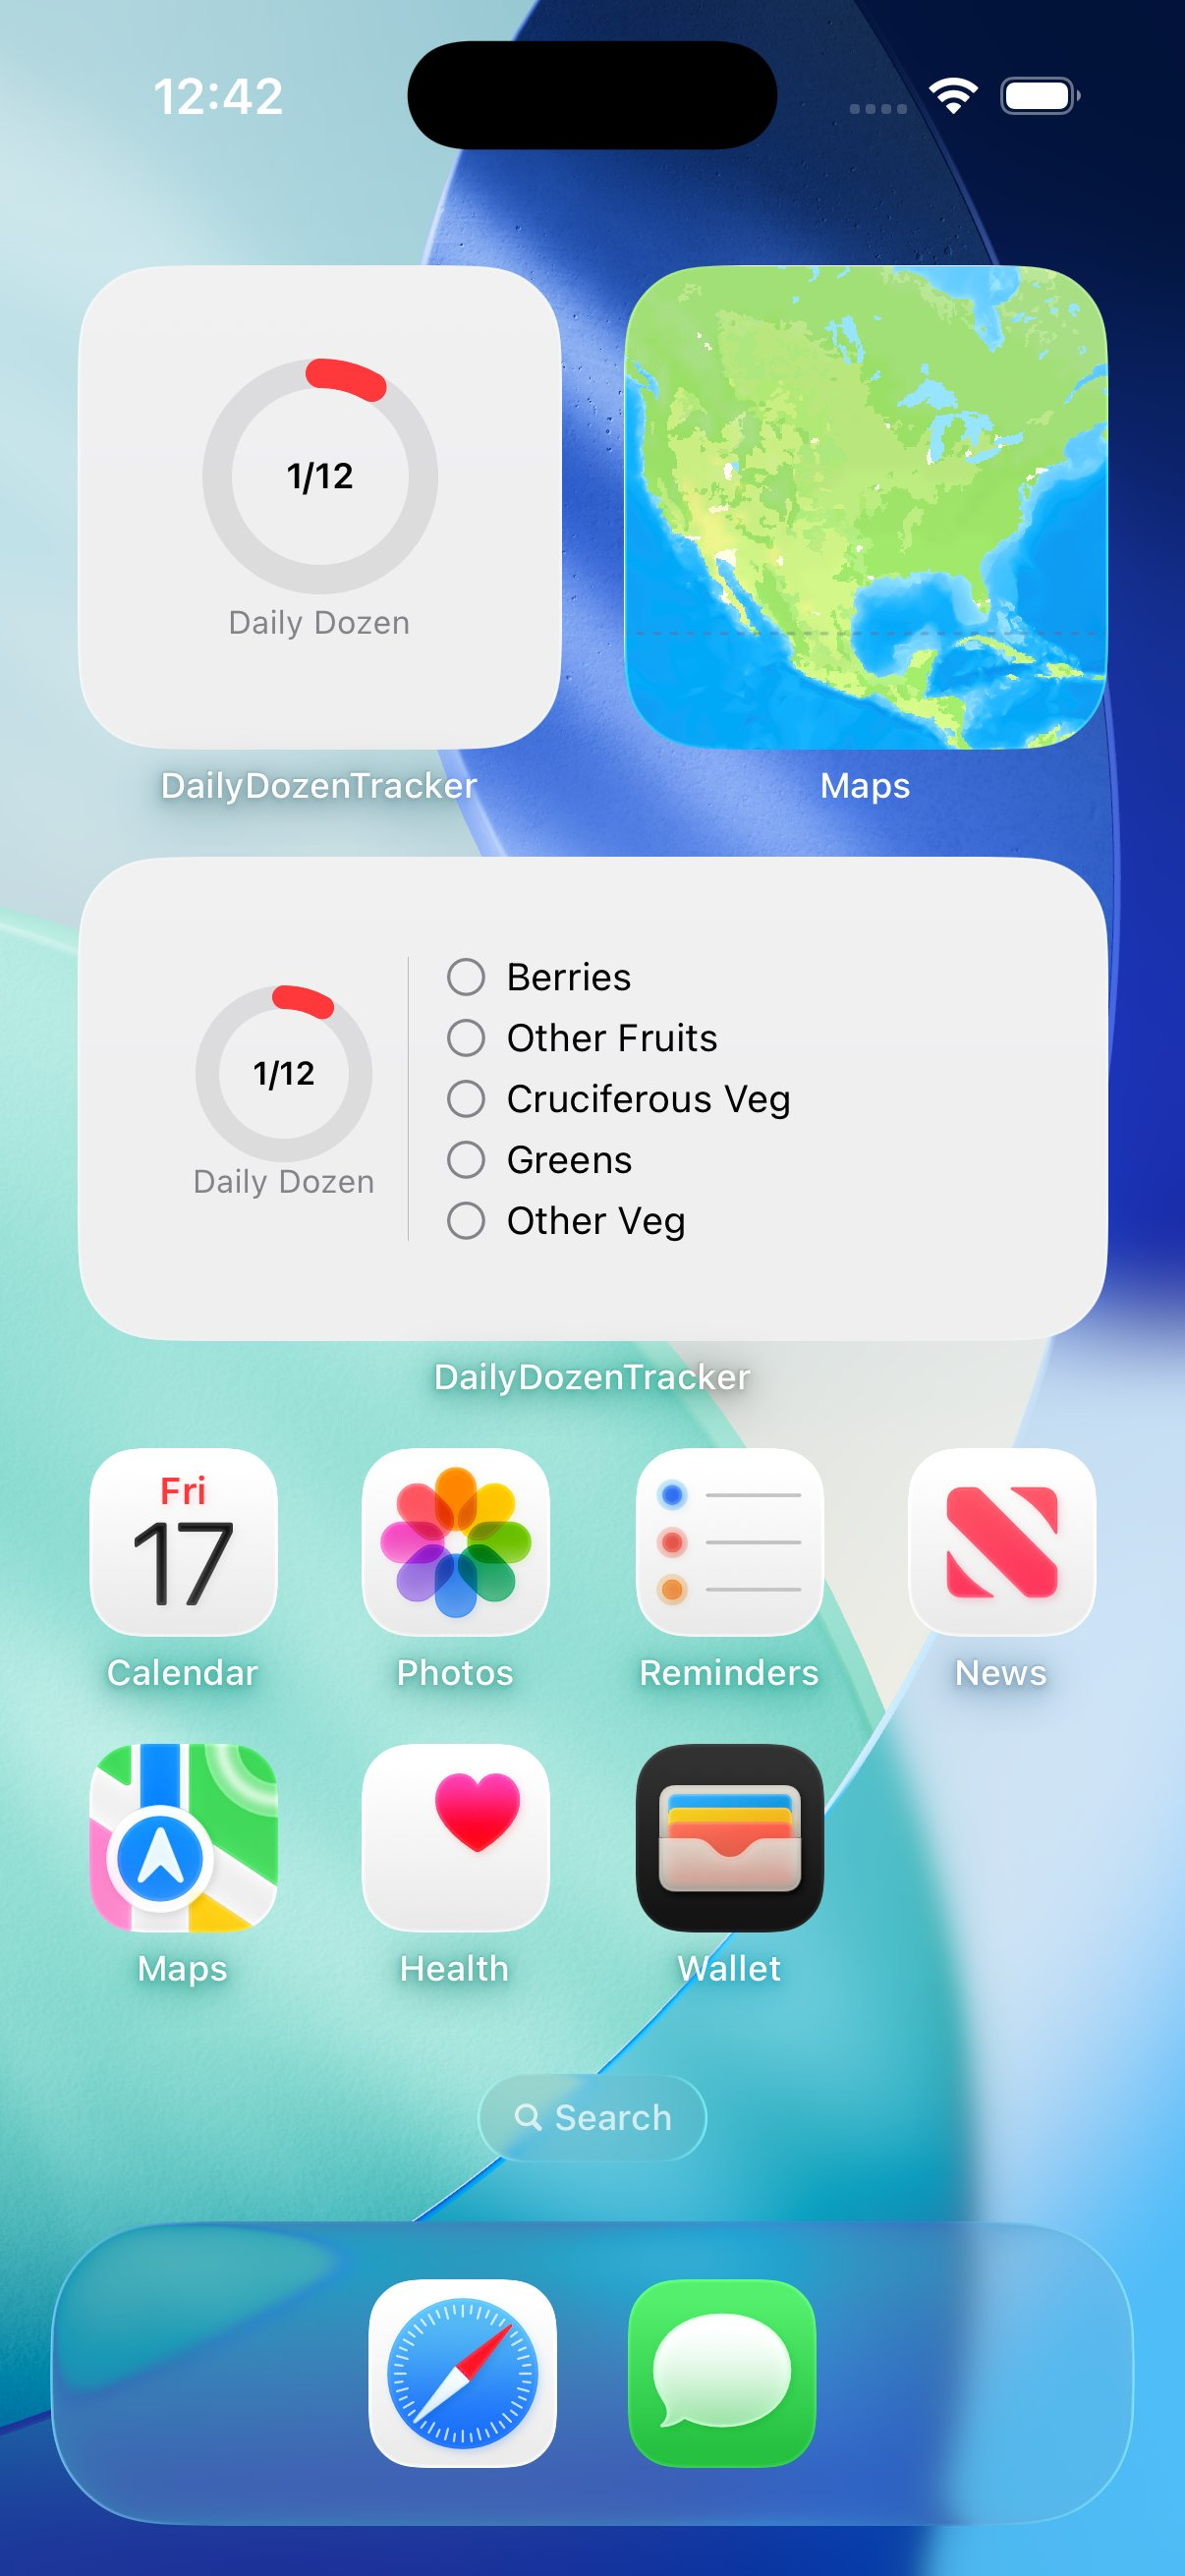
\includegraphics[width=0.32\linewidth]{home_screen_early.png}\hfill
    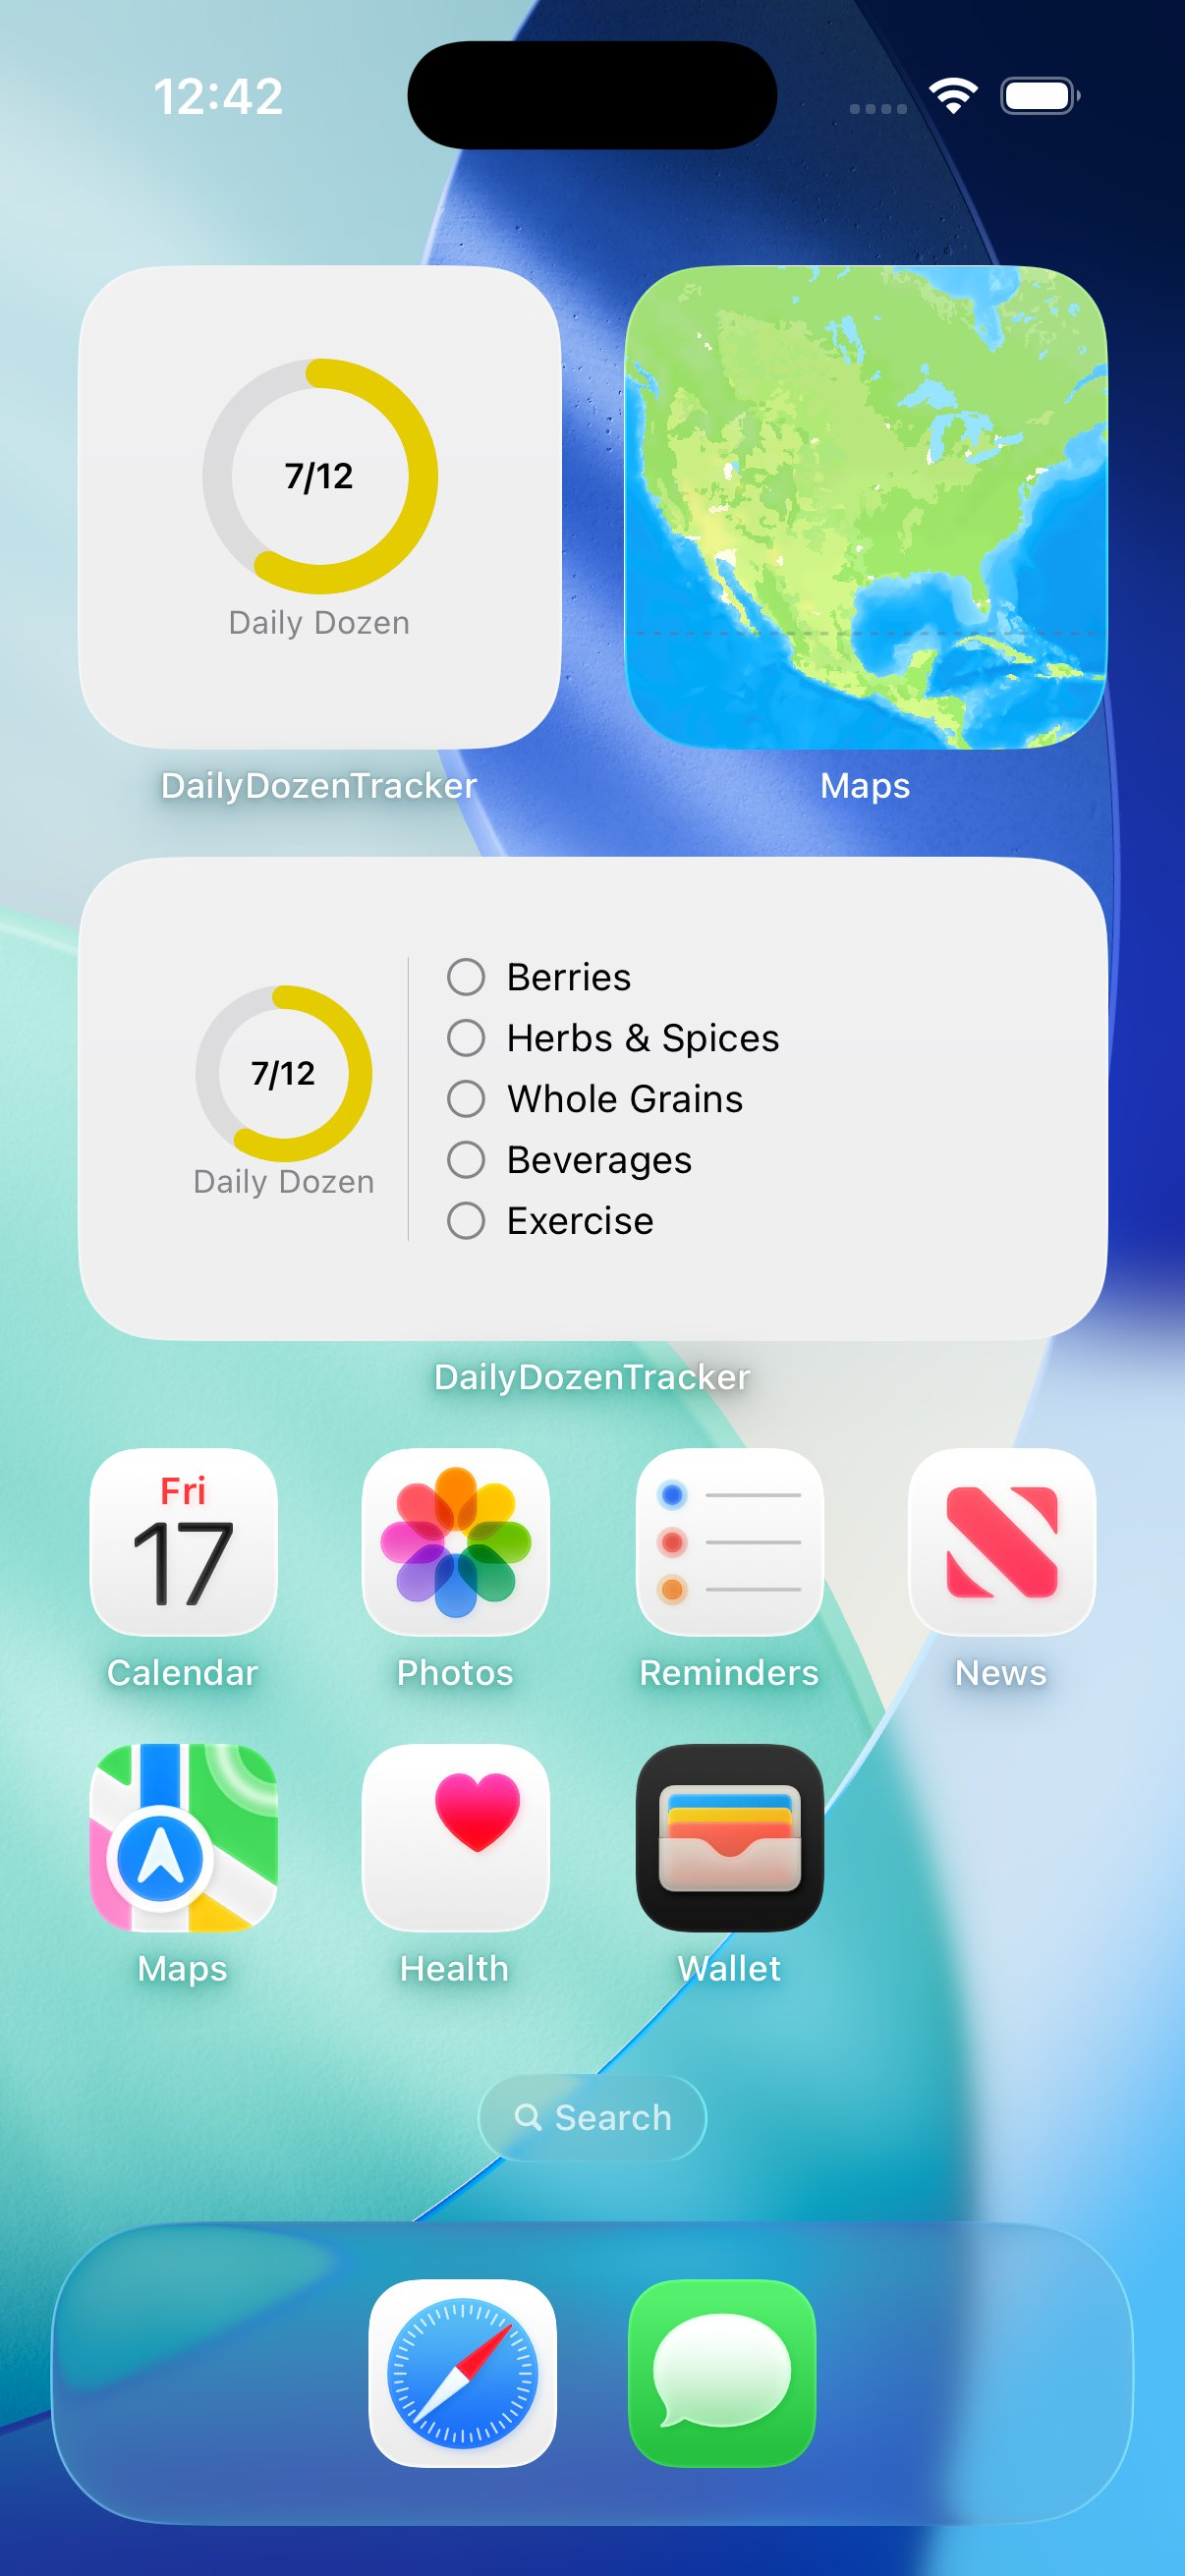
\includegraphics[width=0.32\linewidth]{home_screen_mid.png}\hfill
    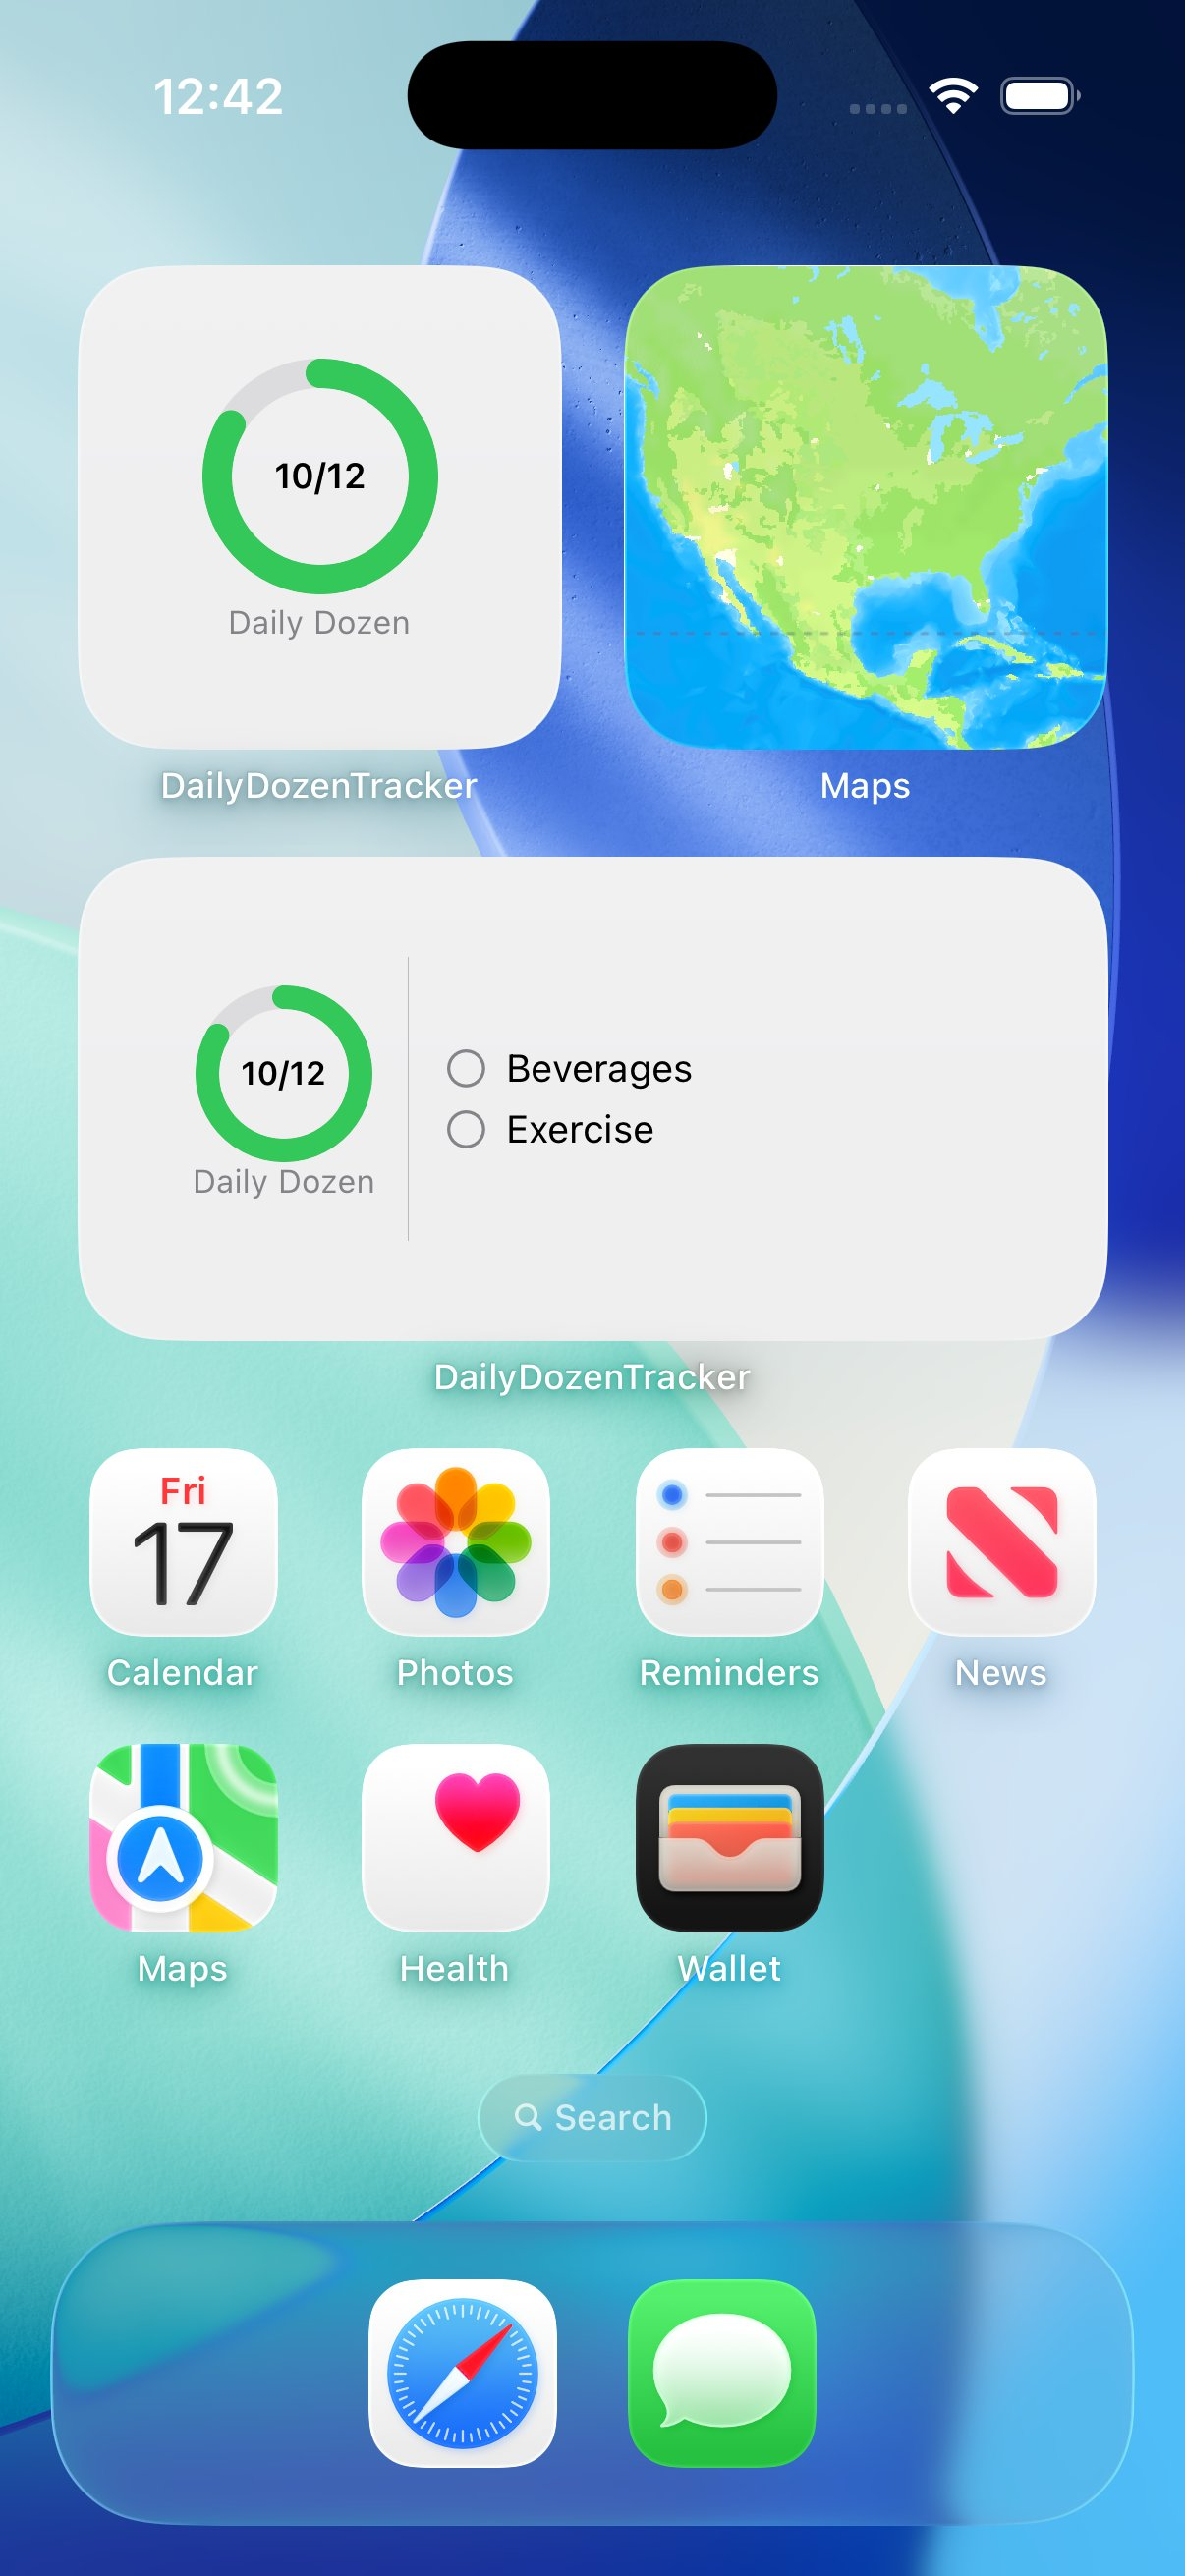
\includegraphics[width=0.32\linewidth]{home_screen_late.png}
    \caption{The Small (\texttt{systemSmall}) and Medium Home Screen widgets at three progress states: 1/12 (red), 7/12 (yellow), and 10/12 (green). The color-coded ring gives an immediate progress signal without requiring the user to read the numeric label. The Medium widget surfaces up to five unchecked categories at a time, and rotates a new category into the slot whenever one is completed. Both sizes are view-only; tapping opens the app rather than logging in-place.}
    \label{fig:homescreen_widget}
\end{figure}

\begin{figure}[t]
    \centering
    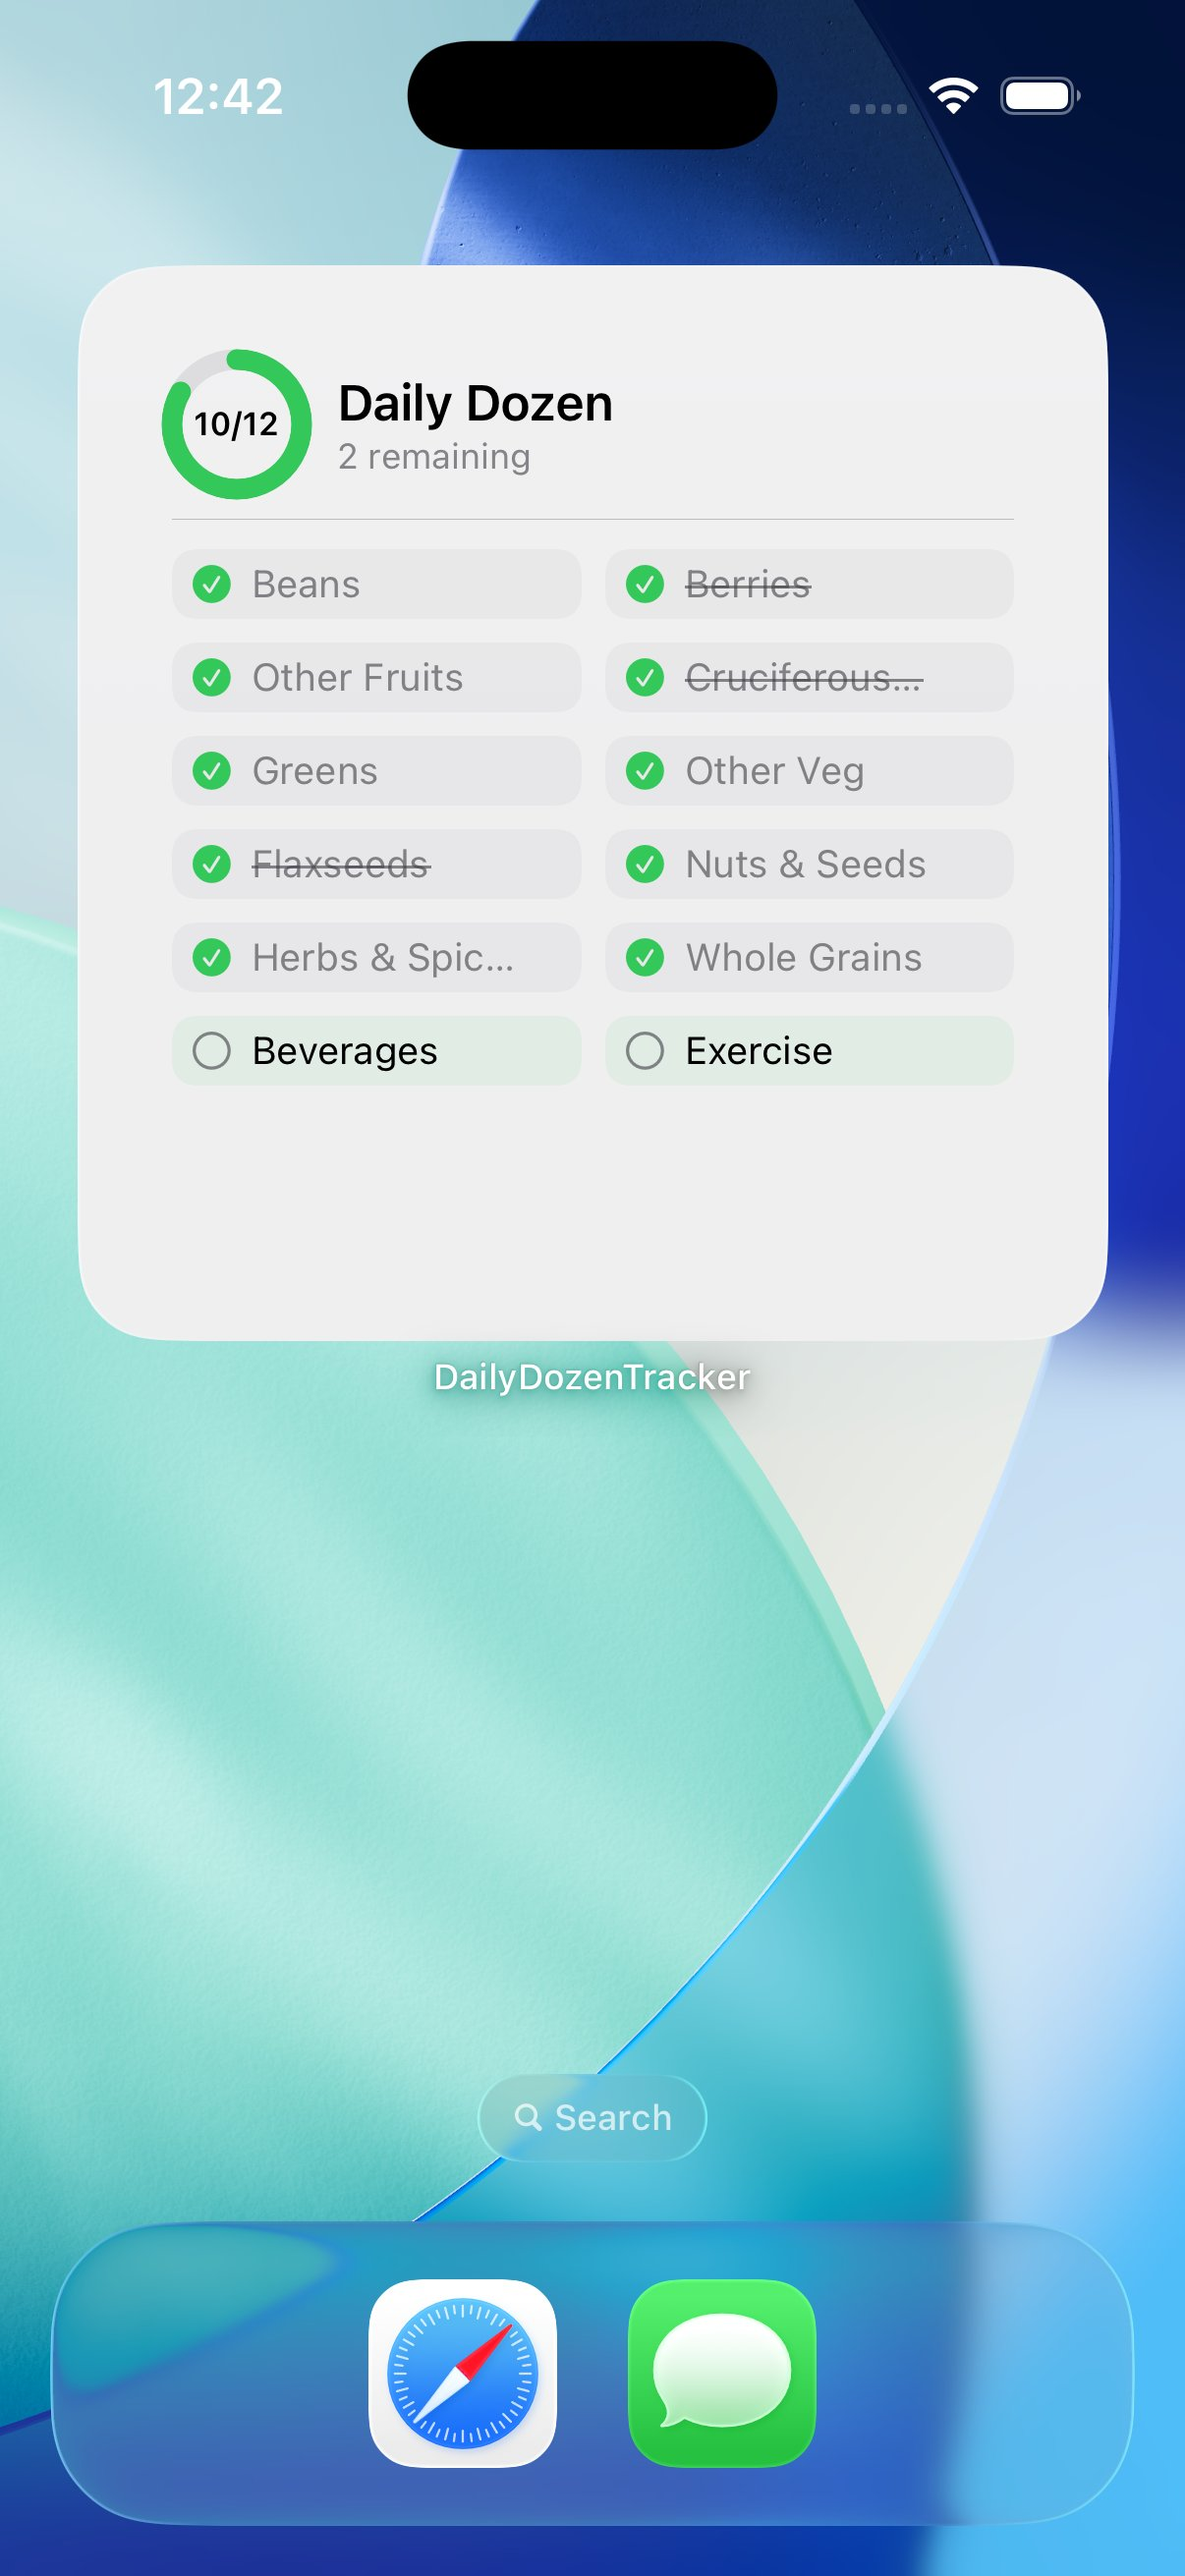
\includegraphics[width=0.70\linewidth]{home_screen_large.png}
    \caption{The Large (\texttt{systemLarge}) Home Screen widget at 10/12 completion. All twelve categories are visible in a two-column grid; completed items show a green checkmark, incomplete items remain tappable. This is the only Home Screen configuration that exposes the full checklist without scrolling.}
    \label{fig:homescreen_large}
\end{figure}

\subsection{Lock Screen Widget}

The Lock Screen widget is entirely view-only. Its only job is to let users check their daily progress without unlocking the phone at all. That came out of participant feedback: they said that unlocking the device, even with Face ID, was enough of a context switch to pull them into notification badges and adjacent app icons and distract them. Putting the progress ring on the Lock Screen sidesteps that.

The widget shows the same progress ring and counter as the Small Home Screen widget (e.g., ``3/12''), but it's set up with a separate WidgetKit configuration that targets the \texttt{.accessoryRectangular} and \texttt{.accessoryCircular} complication families Lock Screen widgets use. Lock Screen widgets can't fire App Intents in the same backgrounded way Home Screen widgets can, so I deliberately left interactivity out. The Lock Screen handles awareness; the logging itself is handled on the Apple Watch or the Medium/Large Home Screen widget.

\begin{figure}[t]
    \centering
    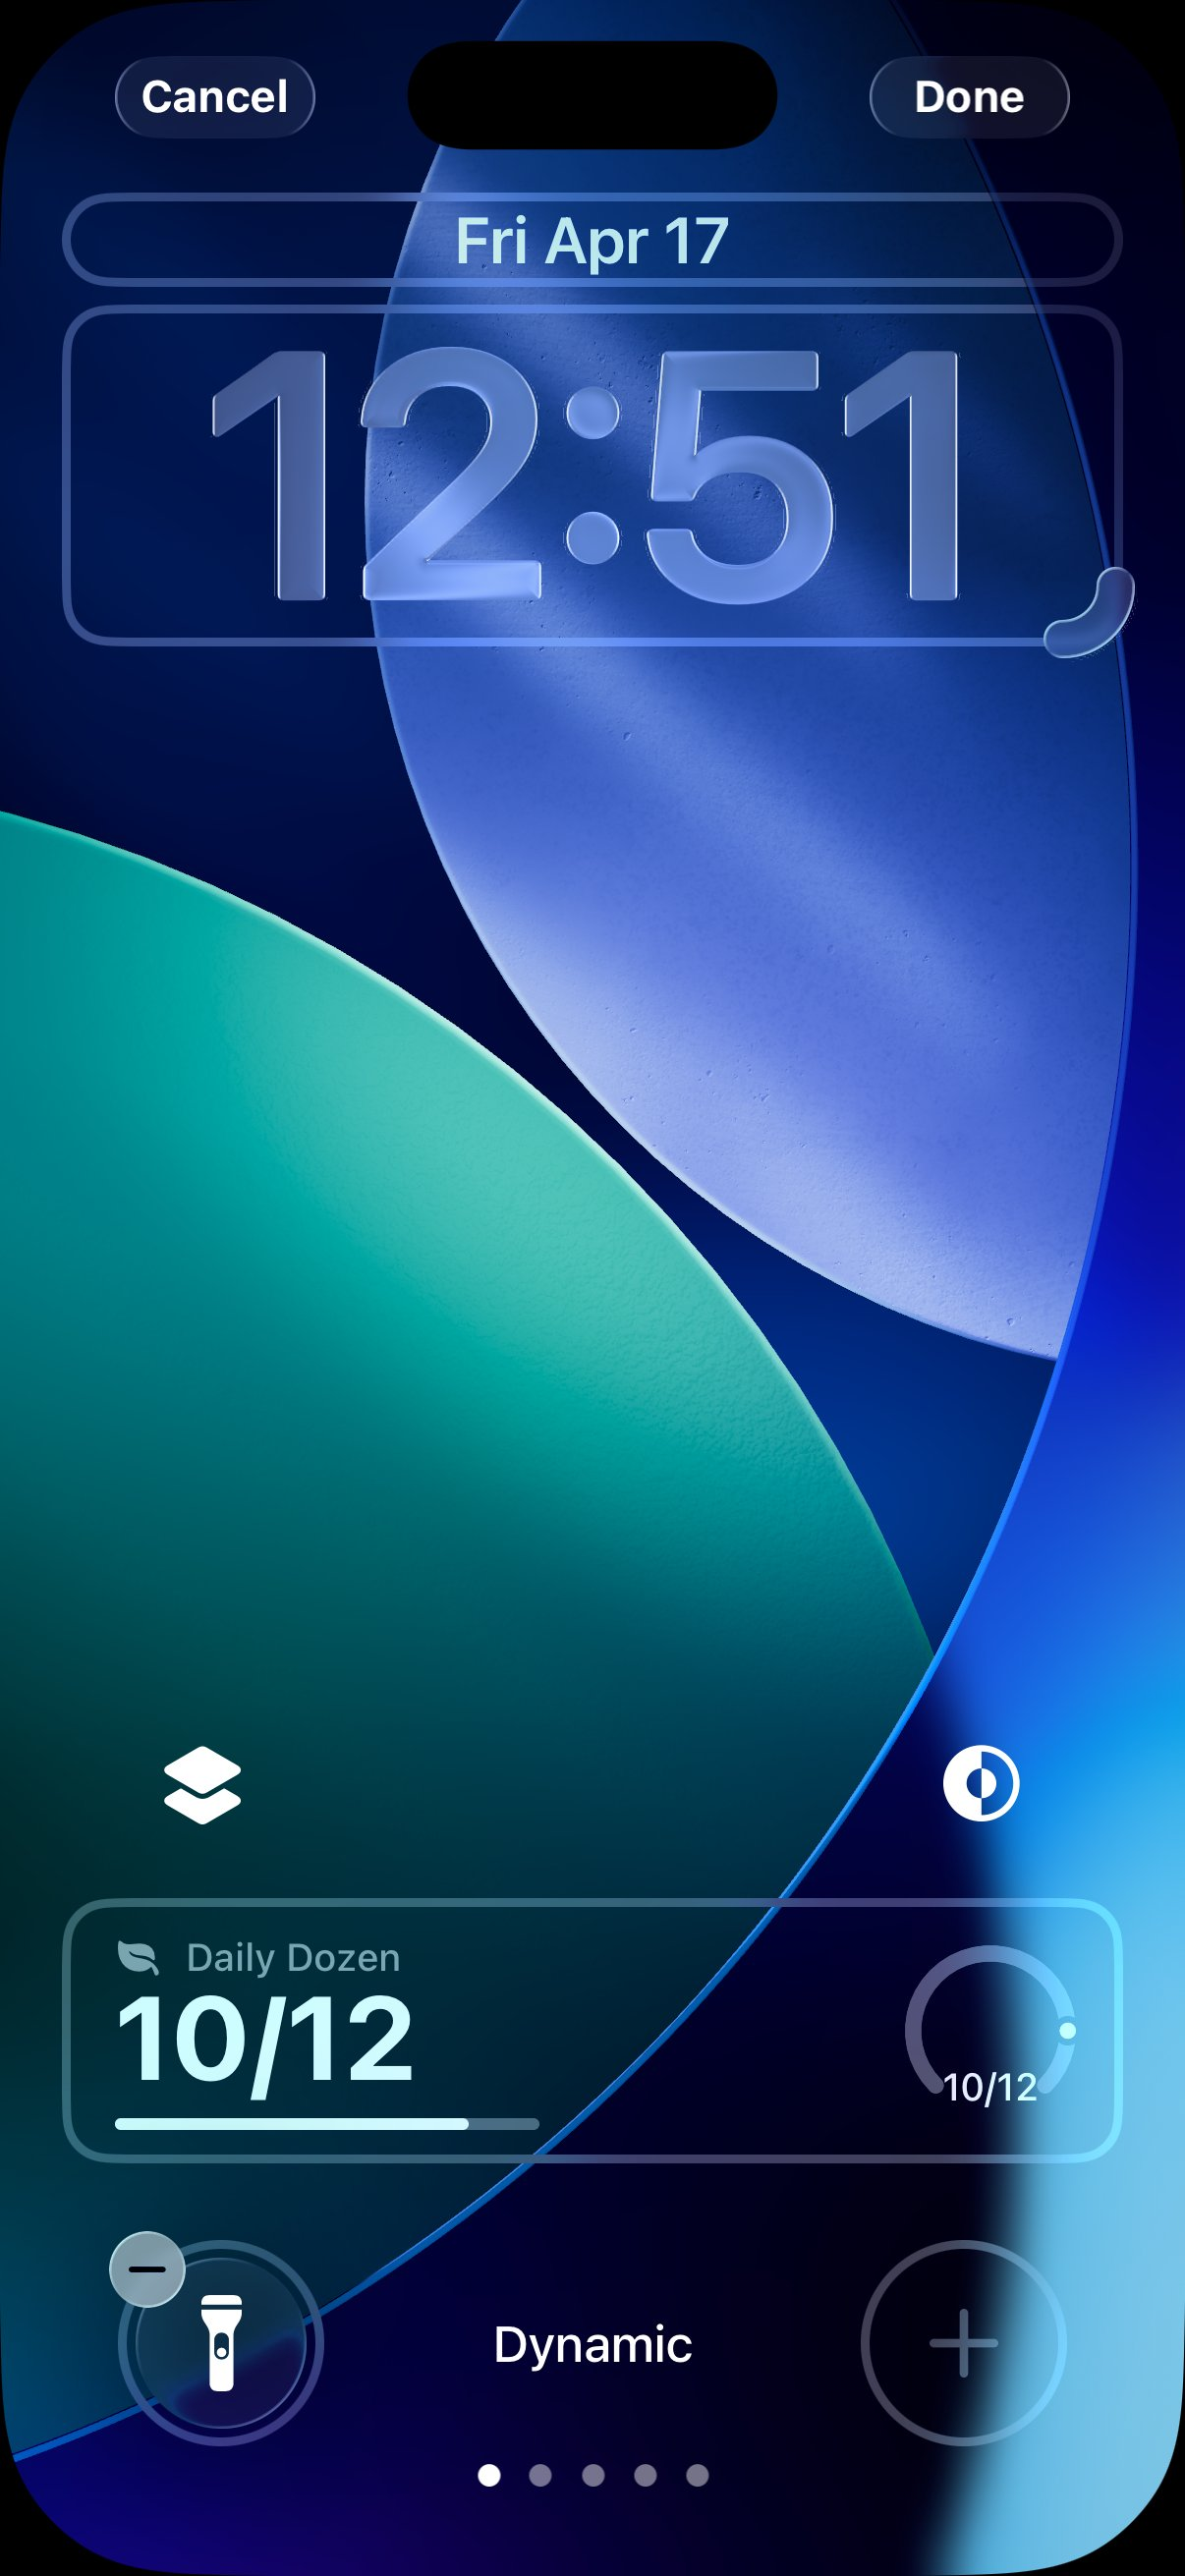
\includegraphics[width=0.55\linewidth]{lock_screen_widget.png}
    \caption{The Lock Screen widget in customization mode, showing both supported complication families. The \texttt{.accessoryRectangular} widget (bottom-center) displays the app name, a bold numeric counter (e.g., ``10/12''), and a linear progress bar. The \texttt{.accessoryCircular} widget (bottom-right) renders a compact arc ring with the same counter. Both are view-only; the user can check status without unlocking the device.}
    \label{fig:lockscreen_widget}
\end{figure}

\subsection{Apple Watch Complication}

The Apple Watch has the least screen real estate of any of these surfaces, and trying to cram twelve interactive buttons onto it would have needed scrolling, which defeats the whole point of a glanceable interface. So I used the \texttt{.accessoryCircular} complication family and went with the Progress Gauge approach again: a dynamic ring plus a counter (e.g., ``3/12''). What the user sees on their wrist is basically a yes/no answer to ``Am I done for the day?'' The Watch's constraints forced me into this reduced view, but there's an upside. An incomplete ring still acts as a psychological nudge.

\begin{figure}[t]
    \centering
    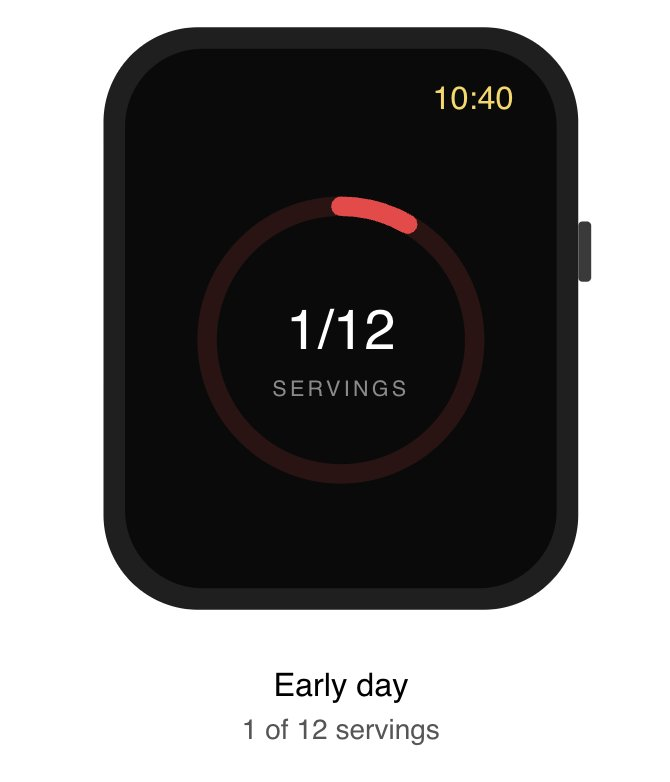
\includegraphics[width=0.48\linewidth]{watch_early_day.png}\hfill
    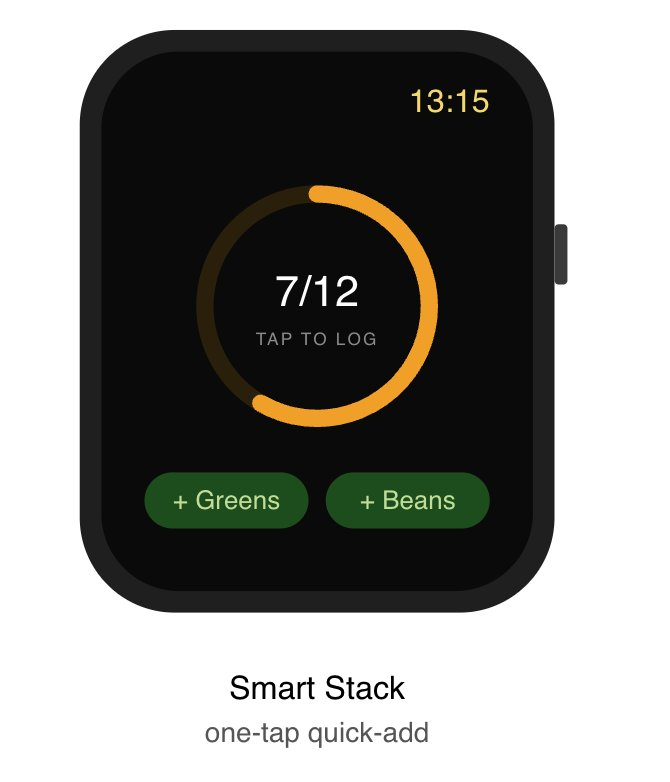
\includegraphics[width=0.48\linewidth]{watch_smart_stack.png}
    \caption{The Apple Watch complication in two configurations. Left: the view-only \texttt{.accessoryCircular} complication at 1/12 completion (early day, red), abstracting the full checklist into a single glanceable metric. Right: the Smart Stack variant surfaces two predicted quick-add pills (``+ Greens,'' ``+ Beans'') alongside the ring, enabling single-tap logging without launching the full app---a direct implementation of the time- and location-aware prediction described in Section 8.2.}
    \label{fig:watch_complication}
\end{figure}

The Apple Watch complication is the only surface that does both glanceability and logging. Tapping the complication fires an App Intent in the background, bumps the relevant category counter, and calls \texttt{WidgetCenter.shared.reloadAllTimelines()} to refresh the ring immediately. If the user has the Always-On display turned on, they don't even need to wake the watch. Total interaction cost is one tap.

\subsection{Participants}

I recruited a convenience sample of eight participants from the undergraduate student body, ages 18 to 22. I picked this group specifically because they're the people who grew up with smartphones and are fluent with mobile interfaces, but also the people who most frequently complain about notification fatigue and dropped apps. Three of them wore an Apple Watch daily, which gave me a small subset for the wearable analysis. Only one was strictly vegan, but all of them said they wanted to eat more fruit and vegetables. That last part mattered. Participants who don't care about tracking their diet would have been measuring forced compliance, not actual usability.

\subsection{Apparatus and Environment}

I ran the tests in a controlled lab setup, but designed the tasks to mimic real-world distraction. Participants used an iPhone 15 Pro Max so that screen size and processing speed stayed consistent across trials. Watch testing was done on an Apple Watch Series 9. Both devices came pre-loaded with two things: the standard Daily Dozen app (version 3.0), which served as the control, and my custom ``Widget-Dozen'' TestFlight build as the experimental variable. Based on what came out of the formative survey, the experimental build used the ``Status-Only'' configuration: a simple ``0/12'' progress ring, not the quick-add buttons I'd initially planned. To approximate the physical effort of starting a logging task in real life, I put the phone face-down on the table before each trial, so the user had to pick it up before they could do anything.

\subsection{Procedure}

The study used a Within-Subjects design: each participant tried both the control (standard app) and the experimental condition (widgets), so I could compare them directly. I counterbalanced the order of the conditions to control for learning effects. Each session opened with a five-minute onboarding where I walked the participant through the Daily Dozen idea and the specific food categories they'd be logging.

The first task was the ``Cold Log,'' the control condition. I gave them a scenario, e.g., ``You just finished a salad with spinach and chickpeas,'' and asked them to log one serving of Greens and one of Beans using the standard app. I timed the interaction from the moment their hand touched the phone until they put it back down on the table. The second task repeated the scenario, but using the interactive Home Screen widget. Last was a ``Glance Test,'' where I asked them to check their progress using the Lock Screen widget versus opening the app. The session ended with a semi-structured interview about their experience, specifically about the ``annoyance factor'' of each method, and any sense of being ``nagged'' by either one.

\section{EVALUATION METRICS}

To turn the vague idea of ``user needs'' into actual data, I picked metrics from HCI theory, mainly the Keystroke-Level Model (KLM) and Cognitive Load Theory.\cite{CardKeystrokeModel}

\subsection{Primary Metric: Interaction Steps}

I defined an ``interaction step'' as any motor action that advances the system's state: physical button presses, screen taps, swipes, or a successful Face ID unlock. I picked this as the primary quantitative metric based on the GOMS (Goals, Operators, Methods, Selection rules) model, which says the reliability of a routine behavior is inversely proportional to the number of steps it takes. For habit formation, every extra step is another chance for the user to give up. Counting steps is basically counting how likely the behavior is to happen at all, so a lower step count should, in theory, mean better long-term adherence.

\subsection{Secondary Metric: Time-on-Task}

My secondary quantitative metric was Time-on-Task, measured in seconds from the moment the user reached for the phone to the moment they saw the checkmark appear. Milliseconds always matter in interface design, but here Time-on-Task is really a stand-in for what I'd call the ``Interruption Factor.'' A fifteen-second task interrupts whatever social or work activity the user was doing. A two-second task is a micro-interaction that can happen mid-conversation or mid-walk. My goal was to get Time-on-Task below the point where it feels like task-switching at all.

\subsection{Qualitative Metrics: Cognitive Load and Prospective Support}

For the mental effort side of things, I used a Perceived Cognitive Load metric based on a modified ``Single Ease Question'' (SEQ) approach. People usually ditch apps because they find them mentally exhausting, more than because they find them physically hard to use.\cite{AppleHIGWidgets} Navigating an app hierarchy means doing ``wayfinding,'' holding a mental model of where you are and where you're going. Tapping a widget just requires recognizing the right thing on the screen. I wanted a way to measure that mental overhead, since the physical step count alone doesn't capture it. I also measured Prospective Support (``Glanceability'') as a simple yes/no: could the user check their status without touching the device? Since prospective memory falls apart without a cue, the ring needed to be a good enough visual prompt to count as one.

\subsection{Rejected Metrics}

I considered a few other metrics but decided against them. Daily Active Users (DAU) and Retention Rate are standard for app success, but both need a longitudinal study running over weeks or months to mean anything.\cite{MatthewsGlanceability} That wasn't going to fit inside an academic semester. I also skipped Caloric Accuracy. A lot of health studies measure how precisely users log their food, but the Daily Dozen is a checklist, not a calorie calculator, so input precision wasn't a variable that mattered here.

\section{RESULTS AND DISCUSSION}

Data from the eight participants backs up the hypothesis that cutting OS-level friction makes health tracking easier to stick with. The widget condition beat the control on every metric I measured.

\subsection{Quantitative Analysis: The Efficiency Gap}

The step-count difference was big and consistent across all eight participants, which lines up with the ``Ability'' part of Fogg's Behavior Model.\cite{FoggBehaviorModel} The standard-app condition took 5.2 steps on average: wake the phone, swipe to find the app, tap to launch, wait through the splash screen, scroll to the category, and tap to log. The widget condition took just 2.0 steps (wake, tap). For users with the Apple Watch Always-On display turned on, it was one step, because the wake was passive. That's a 61.5 percent reduction in steps for phone users and an 80 percent reduction for Watch users.

Time-on-Task told the same story. The standard app took 8.4 seconds on average, with a standard deviation of 1.2 seconds. The widget averaged 2.1 seconds with a standard deviation of just 0.4. That's a 75 percent cut, and it changes the character of the interaction. At 8.4 seconds, logging is a task: you have to stop whatever you were doing to do it. At 2.1 seconds, it's a gesture you can fit into the middle of a conversation or a walk. The lower standard deviation on the widget side also suggests the widget is more predictable, with less room for user error or system lag.

\subsection{Thematic Analysis of User Interviews}

I coded the qualitative feedback into three themes that help explain the ``user needs'' behind the numbers.

The first theme was what I started calling the ``Social Cost'' of tracking. I didn't expect this one. Several participants said that unlocking their phone and navigating to an app while they were eating with friends felt rude. It looked the same as checking texts or social media. The Lock Screen widget plus the Apple Watch tracker fixed this. Glancing at a progress bar on the Lock Screen or discreetly tapping the Watch to log a serving was subtle enough to do at a dinner table without derailing the conversation. ``Discreetness'' as a user need doesn't come up much in existing health app research, as far as I can tell.

The second theme was what I'd call ``Object Permanence'' for habits. Participants described the old app as out of sight, out of mind. They'd forget it existed until a push notification hit them late in the day. The Home Screen and Lock Screen widgets changed that. By taking up real pixels on the device, the Daily Dozen stopped being something you had to remember and started being part of the environment. The visible progress ring worked as a passive prompt: people said seeing an incomplete bar on their Home Screen made them want to ``close the ring'' by tapping their Watch. That's the Zeigarnik Effect in action, where unfinished tasks nag at you,\cite{ZeigarnikEffect} and it works without any push notifications.

The third theme was ``Friction as a Motivation Killer.''\cite{LiPersonalInformatics} Even small amounts of friction turn out to kill adherence way out of proportion to how small they are. One participant told me that opening the app to check their progress usually led to them noticing a text or email, which then pulled them off-task and made them forget why they'd opened the phone in the first place. Context switching was doing the damage. The view-only widgets act as a kind of ``Protective Filter'': the user can check their status on the Lock Screen without ever unlocking the device. Keep the actual logging on the Watch, keep the phone locked, and you avoid the doom-scroll that tends to follow any unlock.

\subsection{Caveats and Alternative Explanations}

The results look good, but I should flag some alternative explanations. One is the Novelty Effect: maybe people liked the widget just because it's new and visually interesting. I don't think that fully explains it, though. The specific pain points participants brought up (social anxiety, distraction) point to real utility beyond the appeal of something new. I also want to be honest about where this solution hits its ceiling. The Daily Dozen is a simple boolean checklist, which is a good fit for a widget.\cite{GregerHowNotToDie} More complex tracking tasks, like insulin levels or precise food weights, need a full keyboard, and the widget approach would fail there. So these results really only generalize to ``micro-logging'' tasks, not mobile health apps in general.

\subsection{Connection to Project Goals}

My goal was to cut cognitive friction in health tracking. Step count dropped by over 60 percent and time-on-task by 75 percent. The interview data also shows the intervention worked on the psychological side: the social awkwardness of phone use, the mental overhead of remembering. For habit-forming apps, pulling the interface out to the OS surface layer seems to be what actually bridges intention and action.

\subsection{Observational Finding: Digital Distraction}

One thing I didn't quantify but noticed a lot was how easy it was for participants to get distracted during the control trials. On three separate occasions, participants who unlocked their phone to open the standard app got sidetracked by a notification badge on a messaging or social media app before they could find the Daily Dozen icon. That's the cognitive cost of navigating the OS's ``attention economy.''\cite{HayesSirensCall} The view-only widget skips past this entirely: you check your progress on the Home Screen without entering the app grid, so you never have to swim through the notifications.

\subsection{Limitations}

The step-count reduction is objective, but my sample was small (n=8) and all college students. Older adults or less tech-savvy users might find setting up widgets in the first place to be its own barrier. All the usability trials also ran on the Xcode iOS Simulator, not on real hardware. This hits the Apple Watch part the hardest: using a mouse pointer to poke at a simulated digital crown doesn't really replicate the ergonomics, haptics, or lift-to-wake timing of an actual wrist device. And the study measured discrete simulated tasks, not whether people actually stick with the habit over time. The obvious next step is deploying on physical devices and running a longer study to see if the theoretical friction reduction actually moves the needle on dietary adherence over months.

\section{FUTURE WORK}

\subsection{Platform Expansion and Ecosystem Continuity}

This study focused on iPhone and Apple Watch, but the Daily Dozen isn't really tied to either.\cite{GregerHowNotToDie} A good next target would be macOS desktop widgets.\cite{AppleHIGWidgets} For anyone who spends their workday at a computer, the phone is a distraction vector; a desktop widget would let them log lunch without having to look away from their main workflow. The other interesting angle is iOS 17's ``Standby Mode,'' which turns the iPhone into a smart display when it's charging horizontally. A ``Kitchen Display'' mode of the widget, designed to be readable from across the room while you're cooking, would put the tracker right where the behavior actually happens.

\subsection{Automated Intake via Shortcuts and AI}

What I built cuts physical friction, but users still have to tap things themselves. The obvious next step is cutting cognitive friction through automation. Exposing the widget's ``Log Item'' actions to Apple's Shortcuts app would let users set up things like ``When I get to Sweetgreen, remind me to log Greens.'' On-device machine learning via CoreML could go further and predict what the user is likely to log based on time of day and location, surfacing ``Oatmeal'' at 8 AM and ``Legumes'' at noon, which would cut out the step of finding the right category at all.

\section{ETHICAL CONSIDERATIONS}

The project is trying to improve health outcomes, but any tool that encourages obsessive tracking has ethical risks worth flagging.

\noindent\textbf{Data Privacy:} The widget system handles some pretty personal health data, so I kept everything local, using Apple's HealthKit and on-device storage.\cite{AppleHIGWidgets} No data gets sent to any external cloud server; every Daily Dozen log stays on the user's device. That ``local-first'' setup means a user's dietary habits can't end up getting mined for advertising.

\noindent\textbf{Psychological Impact:} Gamifying diet through always-on widgets could push vulnerable users toward orthorexia or obsessive tracking.\cite{HayesSirensCall} Seeing incomplete dietary tasks sitting on your screen all day could read as pressure rather than support. To keep the design on the supportive side, I avoided red warning-style colors and leaned on neutral or positive feedback (green checks) to frame progress as something to encourage, not something to punish yourself for missing.

\section{CONCLUSION}

Cutting the interaction cost of health tracking seems to matter a lot more than I initially thought, in ways that go past simple convenience. The widget version cut mechanical logging steps by over 60 percent, and the lower step count tracked pretty cleanly with participants saying the tool was more useful. For a habit-forming app, you probably want the interface that demands the least attention rather than the one with the most features. The direction I'd push mHealth work in is away from immersive apps and toward ambient, surface-level interfaces.

\section{REPLICATION INSTRUCTIONS}

To replicate this project or keep developing the artifact, you'll need a Mac running macOS Sonoma 14.0 or later, Xcode 15.0 or later, and a device or simulator running iOS 17. iOS 17 is non-negotiable: the interactive widget code depends on WidgetKit APIs that don't exist in earlier versions.

Start by cloning the project source from the Git repository into a local directory. Open the \texttt{.xcodeproj} file in Xcode and set up signing before you try to build. Under ``Signing and Capabilities'' in the project settings, pick a valid development team. You need to do this for both the main app target (\texttt{DailyDozen}) and the widget extension target (\texttt{DailyDozenWidgetExtension}); if the provisioning profiles don't match, the widget will fail silently at launch.

Once signing is set up, pick the ``DailyDozen'' scheme and a simulator (the iPhone 15 Pro works fine), then build and run. The main app will launch, but the widget won't show up automatically. To get to it, go to the simulator's Home Screen, long-press the background to enter ``jiggle mode,'' tap the plus button in the top-left corner, search for ``DailyDozen,'' and add it to the Home Screen. Tap the interactive elements on the widget to verify that state updates happen in the background without the main app relaunching.

\section{CODE ARCHITECTURE OVERVIEW}

The system is built in Swift 5 with SwiftUI. The core data logic lives in a \texttt{DailyDozensManager} class that conforms to the \texttt{ObservableObject} protocol, so it can broadcast state changes.

\noindent\textbf{Widget Target:} The widget extension uses a \texttt{TimelineProvider} to generate a timeline of \texttt{SimpleEntry} objects. When the user taps a toggle on the widget, it fires an \texttt{AppIntent}.

\noindent\textbf{AppIntent:} I used the \texttt{AppIntent} framework to handle background execution. Its \texttt{perform()} function updates the shared \texttt{UserDefaults} (via App Groups) and calls \texttt{WidgetCenter.shared.reloadAllTimelines()} to refresh the UI right away.

\printbibliography

\end{document}
